\chapter{Implementation}\label{chap:impl}

\guidance{%
  This chapter should describe what was actually produced: the programs which
  were written, the hardware which was built or the theory which was developed.
	Any design strategies that \textbf{looked ahead to the testing stage} might
	profitably be referred to (the professional approach again).\\
  Descriptions of programs may include fragments of high-level code but large
  chunks of code are usually best left to appendices or omitted altogether.
  Analogous advice applies to circuit diagrams.\\ 
  \textbf{Draw attention to the parts of the work which are not your own}. Making
  effective use of powerful tools and pre-existing code is often laudable, and
  will count to your credit if properly reported.\\
  It should not be necessary to give a day-by-day account of the progress of the
  work but \textbf{major milestones may sometimes be highlighted with advantage}.\\
}

\prechapter{%
	Upon completion of the project's plan, its execution commenced. What
	follows is an account of the programs written, problems encountered, solutions
	implemented and tests conducted using the project-structure shown in
	Figure~\ref{fig:structure} as a guide. \emph{Reasons} for design decisions
  (arrived at using \emph{formative} evaluation techniques) are detailed in
  Chapter~\ref{chapter:evaluation} on Evaluation.
}

\begin{figure}[tb]

\centering
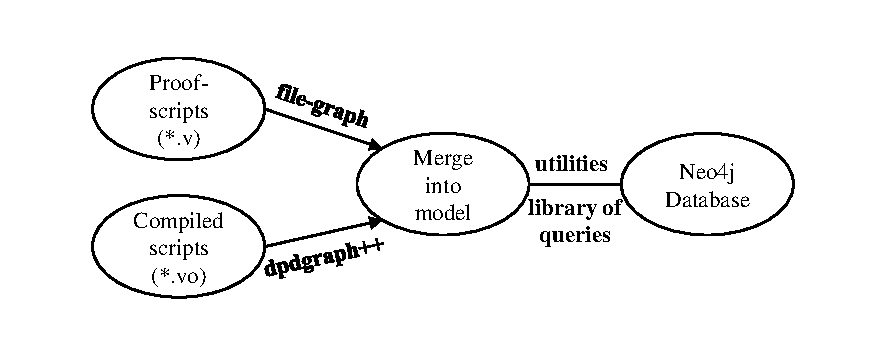
\includegraphics[width=\textwidth, page=1]{proposal/proposal-project-structure-diagram.pdf}
\caption{System Components}\label{fig:structure}

\end{figure}


\section{Coq object-files to CSV}

This section of implementation corresponds to ``dpdgraph++'' on
Figure~\ref{fig:structure}: modelling the data contained in and the structure
of Coq object-files (\texttt{*.vo}) as comma-separated values (CSVs). The
initial model (inherited from the open-source ``dpdgraph'' tool) and subsequent
changes to it will be described.

\subsection{Modelling}

Initially, each edge was assigned a \emph{weight} representing the number of
(directed) uses of one node by another. Each node was assigned four
\emph{properties}: 

\begin{itemize}
  \item \emph{body}, a boolean representing whether a global declaration was
    either transparent or opaque;
  
  \item \emph{kind}, a ternary value representing whether a \emph{global
    reference} (a kernel side type for all references) was a reference to either
    the environment, an inductive type or a constructor of an inductive type;

  \item \emph{prop}, a boolean value representing whether a term is a \texttt{Prop}
    (a decidable, logical property about a program, as opposed to a
    general \texttt{Type});

  \item \emph{path}, a string value represent the module an object is in.
\end{itemize}

These properties were difficult to understand: they are not in the
vocabulary of a Coq programmer (e.g. \texttt{Definition}, \texttt{Inductive},
\texttt{Theorem}) and could not represent the richness of the
AST appropriately. It was not documented how to translate these constructs back
to familiar terms and thus, it quickly became clear that the these properties
needed to be replaced by more general and descriptive ones (expounded below).

\subsubsection{Precise Kinds}\label{subsubsec:kinds}

Apart from \emph{path}, all the properties were removed and replaced by two
\emph{labels}: labels are used to group  nodes into subsets; since a node can
belong to more than one subset, it can have more than one label assigned to it.
Implementation of this was simply a matter of looking up and expanding the
abstract syntax tree (AST) starting from the type \texttt{global\_reference}.

The two labels are \emph{kind} and \emph{subkind}.  A \emph{kind} is a string
that can take one of the following values, each directly corresponding to an
AST term: \textsf{module}, \textsf{class}, \textsf{type\_constructor},
\textsf{inductive\_type}, \textsf{definition}, \textsf{assumption} or
\textsf{proof}.

Optionally, some terms have \emph{subkinds}, for distinguishing different
constructs more precisely. For example, when writing Coq, there is no
\texttt{Proof} keyword; instead \texttt{Theorem}, \texttt{Lemma}, \texttt{Fact},
\texttt{Remark}, \texttt{Property}, \texttt{Proposition} and \texttt{Corollary}
all are \emph{synonyms} for proofs. Full details can be found in
Appendix~\ref{chapter:fullmodel}.

\subsubsection{Recursive Modules}\label{subsubsec:recmodules}

What remained from the initial model was the \emph{path} property. The issue
here was that an inherently \emph{hierarchical} structure (of inclusion) was
represented \emph{flatly} as a string attribute of a node. This made modules
second-class citizens, not subject to the same analyses and manipulations as
proof-objects, excluding the possibility of expressing \emph{module-level
dependencies} (as possible in the coqdep tool).

Implementing this feature was difficult; there were two major phases. Firstly,
the type of a node was expanded to include modules (using a variant datatype).
Finishing this involved locating and fixing the resulting type-errors. This
meant modules were in the model, but as a flat structure: modules could be
related to objects but not to other modules.

Thus, the second major phase was inferring and adding all the ``ancestors'' of
a module with the correct relationships (parent as source, child as
destination, repeatedly up to the root module). The initial attempt resulted in
stack-overflow for larger examples. A stack-trace did not highlight any point
of error so it was \emph{assumed} to be due to the na\"{i}ve, but easy-to-write
(and check) non-tail-recursive implementation. So, the code was rewritten in a
space-efficient, tail-recursive manner (which allows for deeply nested module
hierarchies to be handled). Surprisingly, the problem persisted; further
investigation discovered the fault lay in the separate \texttt{dpd2} tool (the
details of which can be found on page~\pageref{subsubsec:dpd2}).

\subsubsection{(Co-)Inductive Types and Constructors}

Now that the properties of the original dpdpgraph had been superseded by more
general and flexible alternatives, it was time to implement new features.  One
of the most obvious and frustrating omissions from the initial model was the
inability to relate an (co-)inductive type to to its constuctor(s). Expanding the
AST term for type-constructors showed which type it constructed (however, types
have no information about which constructors construct them). Hence, since
dependencies were constrcuted in a depth-first manner \emph{down} the AST, they
had to be built in reverse. Therefore, in order to correct this when outputting
edges, each pair of nodes has to be checked to see if it (a) was a type and a
constructor and if so, (b) the constructor's fully-qualified type matched the
fully-qualified name of the type. If both these criteria were met, then the
direction of the edge output was swapped.

\subsubsection{Types}

% Conducting a \emph{cognitive walkthrough} (detailed in
% Chapter~\ref{chapter:evaluation}) spurred the addition of \emph{type
% signatures} to the model.
Type theory is central to a Coq user's work and being
able to include them in the model, would, along with kinds, subkinds and
modules, help towards meeting the modelling requirement~\ref{req:m1} of
including as much relevant data as possible. 

Following the functions called for the Coq command \texttt{Check}
\emph{<expression>} (for printing the type of a given expression) led to the
algorithm for \emph{getting} the type; all that was left was converting the
output to an OCaml string. It was \emph{using} the output which was problematic.
Newlines, quotation marks, and commas had to be replaced by hash signs,
single-quote marks and underscores respectively, so as to not interfere with the
\texttt{dpd} and CSV encoding of data.

\subsubsection{Relationships}

Modelling relationships was the most interesting aspect of deciding how to
represent information. Of primary concern was the notion of expanding a node to
see more details: if a user is looking at an object, they should be able to
expand the object to see what the object depends on; if a user is looking at a
module, they should be able to expand the module to see the objects contained
within that module; if a user is looking at a (co-)inductive type, they should
be able to expand the type and see its constructors. This leads to the basic
modelling structure of \mintinline{cypher}{(src)-[:USES]->(dst)} for
dependencies. For (co-)inductive types, this is refined to a
\mintinline{cypher}{(type)-[:CONSTRUCTED_BY]->(constr)} and for modules this
becomes \mintinline{cypher}{(module)-[:CONTAINS]->(object)}.

Two issues arose whilst implementing these relationships. First, finding and
matching types and constructors (details of which are described earlier).
Second, balancing expressivity against simplicity. Relationships of the
following format, \texttt{X\_USES\_Y} were considered for kinds X and Y.
Although this was useful for fewer kinds, its specificity when subkinds are
included in the model made the model too large and complex (on the order of
$n^{2}$ relationships). Since Cypher allows pattern-matching and filtering
based on kinds and subkinds anyway, this aspect was simplified to the model
presented above.

\subsection{Translation}

Once a model is constructed (in the form of a graph), it is translated by the
\texttt{dpd2} tool to a CSV file for use by Neo4j's import tool to create a
database. An overview of the \texttt{dpd} and CSV formats, as well as the
\texttt{dpd2} tool itself, is presented next.

\subsubsection{\texttt{dpd} Format}

The graph representing the model is output as a \texttt{dpd} file with the
following format for nodes (one per line):

{\tt N: \emph{<id>} "\emph{<name>}" [\emph{<property>}=\emph{<value>}];}

for example (full type elided for brevity), 

{\tt N: 76 "matches" [type="... -> bool", subkind=fixpoint, kind=definition, path="RegExp.Definitions", ];}

and likewise for edges:

{\tt E: \emph{<src id>} \emph{<dst id>} [\emph{<property>}=\emph{<value>}];}

for example, 

{\tt E: 150 145 [type=CONTAINS, weight=1, ];}.

\subsubsection{CSV}\label{subsubsec:translationcsv}

Upon output as as \texttt{dpd} file, a model can be translated to various
other formats. As an example, dpdgraph includes a tool to output a \texttt{dot}
file, used extensively for \emph{visualising} graphs by many tools, from a
\texttt{dpd} file. However, for the purpose of this project, the \texttt{dpd}
file is translated (using the \texttt{dpd2} tool described below) to \emph{two}
CSV (comma-separated values) files: one for nodes and one for edges, for use
with Neo4j's import tools, with the following headers.

{\tt objectId:ID(Object), name, kind:LABEL, subkind:LABEL, path, type}

Here we see name, path and type declared as properties, kind and subkind
declared as labels and the objectId field declared as unique identifier (or in
relational terms, a key) for the nodes (in this schema, called ``Objects'') in
the graph.

{\tt :START\_ID(Object), :END\_ID(Object), weight:int, :TYPE}

Similarly, here we see relationships (between ``Objects'' as declared
previously) named according to the value under the \texttt{:TYPE} column (e.g.
\texttt{CONTAINS}, \texttt{USES} or \texttt{CONSTRUCTED\_BY}), each with an
integer property, weight.

By using a CSV format, adding extra properties, labels and relationships becomes
very straightforward and allows for easy integration (with external tools) and
extension for new features.

\subsubsection{\texttt{dpd2} Tool}\label{subsubsec:dpd2}

Initially, this tool started out as the \texttt{dpd2dot} utility (bundled with
dpdgraph), refactored into \texttt{dpd2csv} which output CSVs instead. Later,
both were combined into a more general, \texttt{dpd2} tool which could accept
the file-type as a command-line argument. As mentioned
in~\ref{subsubsec:recmodules}~\nameref{subsubsec:recmodules} on
page~\pageref{subsubsec:recmodules}, a stack-overflow error occured because of
this tool. By default, \texttt{dpd2} attempts to remove reflexive and
transitive dependencies (i.e. $a \rightarrow a$ and removing $a \rightarrow c$
if $a \rightarrow b$ and $b \rightarrow c$) in a depth-first manner.  For large
graphs, doing so is stack-intensive, and thus causes the aforementioned error.
Since this ``feature'' was unnecessary (because it \emph{removed} useful
information) and appeared time-consuming to fix, the \texttt{-keep-trans} flag
was passed on subsequent uses to avoid the issue altogether.

\section{Coq source-files to CSV}

This section of implementation corresponds to ``filegraph'' on
Figure~\ref{fig:structure}: modelling the data contained in and the structure of
Coq source-files (\texttt{*.v}). First, deficiencies with the model so far
(relying only on information from \texttt{*.vo} files via ``dpdgraph++'') are
mentioned. Then, attempts to address those deficiencies are described. Finally,
conclusions regarding the practicality, necessity and contribution of
``filegraph'' to the overall project are drawn.

\subsection{Deficiencies in the Model}

Some small issues remained with the model as presented so far: \emph{apparent}
absence or duplication of some modules and a lack of notation and tactics.
Oddities with modules arose from the use of \emph{functors}: modules that take
other modules as arguments (used to abstract over agruments, tactics,
defintions and proofs).

A concrete example (from the Coq Standard Library) is the theory of total
orders, minimums and maximums, which is applied to naturals, integers and
rational numbers (as well as any further ordered types). Such functors cannot be
compiled unless fully applied (explaining the \emph{absence} of some modules);
when fully applied, they essentially copy their \emph{structure} into each
instance (explaining the \emph{duplication} of some module names and
structures).

\subsection{Exploring Solutions}

Notation, tactics and functors can all be dealt with by simply parsing
source-files directly with the Coq parser. However, \emph{several issues}
stop this from being a pragmatic solution, least of which are the size of the
AST and complexity of parsing Coq files.

\begin{enumerate}

  \item \emph{Modules and functors are represented identically} in the AST, with
    the former as a special case of the latter, making it very difficult to
    distinguish between the two on an AST-level. By far, this was the biggest
    roadblock.

  \item \emph{Module types}, or \emph{signatures}, must be incorporated into
    the model for functors to make sense. Modules and signatures share a
    many-to-many relationship: a signature can be satisfied by multiple modules
    and a module can satisfy multiple signatures. To express this correctly
    would require \emph{signature-matching}, a notoriously difficult task (and
    the reason why few languages support ML-style modules).

  \item Futher issues involve resolving objects into a global namespace and
    knowing which compiler flags were given during compilation (to match
    physical directories to logical modules), all of which complicate matching
    and merging with the compiled proof objects.

\end{enumerate}

Even though progress had been made tackling these issues, a simpler solution was
desired. \emph{Glob files}, produced during compilation, retain much of the
information in the source code (as a list of globally-resolved names and paths
for each file) in a simpler format. A shell-script was used to prototype a tool
that converted glob files to CSVs. Although promising for tactics and notation,
glob files suffer from the same inability to distinguish between modules and
functors.

\subsection{Resolution}

Both direct-parsing and glob-file approaches to notation, tactics and functors
were limited and time-consuming. Functors are rarely-used with many projects
(especially given the popularity and ease of use of \emph{typeclasses} for
expressing generalisations) and thus risked violation requirement~\ref{req:m1}
(by (a) potentially obfuscating information through their inclusion in the model
and (b) making the model more difficult to use.) Also, in light of
requirement~\ref{req:m3}, given that names \emph{and structures} of instantiated
modules are duplicated, it is possible to \emph{reconstruct} generalisations
\emph{representing functors} once the database is created. As such, extracting
information directly from Coq source-files contributes little to the overall
project, but presents clear ways forward for future-work.

\section{CSV to Neo4j}

As part of the ``utilities'' in Figure~\ref{fig:structure}, Neo4j comes with a
command-line import tool that \textendash~when given a target directory, a CSV
file containing the nodes of the graph and a separate CSV file containing the
edges of the graph \textendash~constructs a database.  As explained
in~\ref{subsubsec:translationcsv}~\nameref{subsubsec:translationcsv} on
page~\pageref{subsubsec:translationcsv}, the headers determine the labels,
properties, IDs of nodes as well as the start- and end-points, properties and
type of edges.

%\subsection{Impact of Changes to Model}
%Trade-offs, execution.

\section{Query Library}

Finally, this last section of the implementation corresponds to the ``library of
queries'' shown in Figure~\ref{fig:structure}. Extensions, written (in Java and
R) to meet the interaction (\ref{req:i1},~\ref{req:i2},~\ref{req:i3}) and
computation (\ref{req:c1},~\ref{req:c2}) requirements on page~\pageref{req:i1},
and their uses are outlined.

\subsection{Java Library}

Briefly, APOC (Awesome Procedures on Cypher) provides, out of the box (by
placing a jar file into a database's plugins directory), many convenient,
utility functions to use. Of note are:

\begin{itemize}

  \item the ability to examine a \emph{meta-graph} showing which labels and
    relationship-types are available in the database and how they are connected, 
    allowing a user to see an overview of the model;

  \item a few key graph algorithms, such as node and path expansion, spanning
    tree, Dijkstra's shortest paths, A*, label propogation (for community
    detection), centrality measures (betweenness and closeness) and PageRank;

  \item some utility functions for regular-expressions and mathematics, useful
    for selecting nodes based on statistics (e.g. PageRank) or selecting nodes
    based on their path.

\end{itemize}

Each of these can be called directly from within Cypher; for example, writing
\texttt{call apoc.meta.graph()} would return the meta-graph of the database.

\subsubsection{Additions}

APOC is used as a foundation for simpler, domain-specific query library.  As an
example, a user can write \texttt{coq.assumptions(<node>, <depth>)} to examine
the n\textsuperscript{th} level assumptions behind a given node. More
convenience functions are defined for executing some of the listed algorithms on
all nodes in a given module or of a given type. For more complex, efficient and
scalable/scriptable analyses however, igraph and R must be used.

\subsection{R Library}

For the R side of the library of queries, to meet requirement~\ref{req:c1} for
a core set of good, out-of-the-box defaults, several example programs were
written which automatically processed data from a new database, stored the
information again for later use (to avoid recomputation) and output appropriate
visualisations. Since processing could take on the order of minutes, status
updates, informing the user of the task being executed, the time it took to
execute once complete, as well as progress-bars where possible and relevant
(e.g.\ commiting a transaction to the database) were provided.

\subsubsection{Visualisation}

There are many interesting ways to visualise the plethora of data that
analysing large mathematical theories using graph databases makes available.

Simply plotting the density/spread of and correlation between metrics such as
in- and out-degrees, PageRank, centrality measures is a good start and can
occasionally yield useful information. Here, R's strength as a
statistics-oriented programming language shone through, making it easy to
rapidly explore different ideas.

Another, more direct, way of displaying infomation is by displaying the graph
itself. As will be shown in
Section~\ref{sec:libeval}~\nameref{sec:libeval},~\nameref{sec:libeval}, there
are a number of different layouts possible (layered, circular and
force-directed), each contributing to a more comprehensive, overall, picture of
understanding the theory.

Surprisingly, igraph was able to help with this aspect of the project as well.
Whilst visNetwork \textendash~with its own JavaScript, force-directed, physics
rendering \textendash~produced more aesthetically pleasing results for smaller
graphs, the webpages it output for larger graphs took intolerably long to render
inside a typical web-browser (Firefox). Thanks to an (experimental) integration
with igraph (specifically, igraph's layout mechanisms) graph layouts could be
pre-computed in fast, native C/C++.

\section{Project Related}

During implementation, several skills and lessons were learnt about correct
project management. Small things, such as grep-ing a code base or keeping track of
time and a log of work done, proved to be useful. However, to ensure the
project ran smoothly on a larger-scale, the following areas received particular
focus.

\subsection{Testing}

For most of the project, testing was done by manually inspecting output. Though
this was tedious, it was the only way to do so when the model was undergoing
continual development. As soon as the model was settled and focus shifted to
visualisation, automated tests were used (which came in particularly useful when
the project had to be bifurcated to support two different versions of Coq).
Small scripts \textendash~of problems solved when learning Coq \textendash~were
used to check output on a small scale (where every single aspect of a project
was known, and testing turnaround was quick). Coq's Standard Library was used as
a large scale stress-test, to ensure all constructs were translated correctly.
When problems were found, they could usually be traced back to debug output
produced during execution.

\subsection{Continuous-Integration Builds}

Although the project never failed to build locally, there were occasionally
problems when trying to build it on the project supervisor's machine. The
problem was compounded when it became apparent that smaller libraries (such as
CoqRegExp and the solved problems) relied on a version of Coq (8.5.2) older than
the one Mathematical Components (needed for the project's moonshot, the Odd
Order Theorem) relied on (8.6). Setting up Travis-CI for continuous-integration
builds made version dependencies precise and explicit, removing much of the
hassle and uncertainty surrounding builds on other machines.

\subsection{Tooling}

At first, the project was run half on Windows and half on a Linux VM (virtual
machine), using shared folders. There were a number of reasons for this: Coq
and Neo4j were already set up on Windows, both are easier to interact with in a
graphical environment and starting up a VM just for some experimentation
incurred quite an overhead.  Eventually, this set-up became confusing and
time-consuming and a leap to running the project fully on a Linux VM was made.
Nevertheless, issues arose when working on R integrations: running a Java
database inside a Linux VM was insufferably slow, requiring a SSH
reverse-port-forwarding to be set up (to let R inside the Linux VM connect to
a Neo4j instance running directly on Windows) for decent performance.

To be the most productive during longer sessions of work, editor integrations
for OCaml were set up, dramatically reducing the edit-compile cycle (especially
for a strong, statically-typed programming language as OCaml). Coq's use of
non-standard OCaml features, extensions and build-systems became particularly
frustrating at this point. For example, considerable time was spent untangling
the Makefile inherited from dpdgraph to have cleaner, out-of-source builds and
reduce the mess in the current working directory, all to no avail as the
complexity of the build-system became apparent.

\section{Summary}

Just presented was an in-depth account of the programs written (dpdgraph++,
dpd2, Java library, R library), problems encountered (first-class modules,
relating types and constructors, incorporating type signatures, CSV
translation, extracting information directly from Coq source-files, dependency
and version tracking, impenetrable build-systems), solutions implemented and
tests conducted. Where relevant, experiments were mentioned to illustrate
lessons learnt. Throughout, project requirements were referenced to justify
important decisions.
